\documentclass[tikz,border=2pt]{standalone}
\renewcommand{\familydefault}{\sfdefault}
\usetikzlibrary{arrows.meta,calc,positioning}
\tikzset{every picture/.style={line width=1pt, >=Stealth},
         hl/.style={fill=black, fill opacity=0.12, text opacity=1}}
\begin{document}
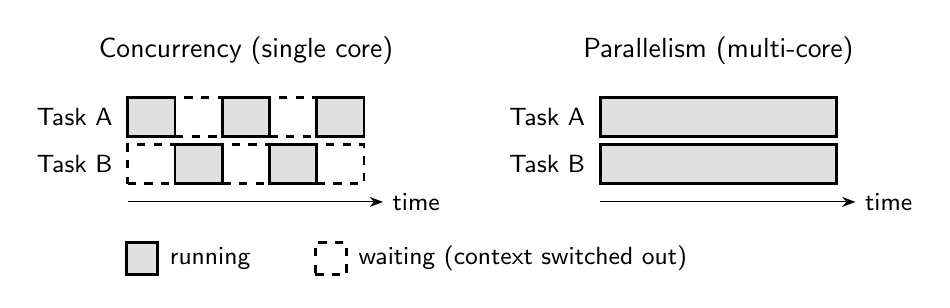
\begin{tikzpicture}[x=0.6cm, y=0.6cm, slot/.style={draw, minimum width=0.6cm, minimum height=0.5cm}]
  % Concurrency: one core alternates between the tasks.
  \node at (2.5, 2.4) {Concurrency (single core)};
  \node[left, font=\small] at (-0.1, 1) {Task A};
  \node[left, font=\small] at (-0.1, 0) {Task B};
  \foreach \i in {0, ..., 4} {
    \pgfmathsetmacro{\a}{mod(\i, 2) == 0 ? "hl" : "dashed"}
    \pgfmathsetmacro{\b}{mod(\i, 2) == 0 ? "dashed" : "hl"}
    \node[slot, \a] at (\i + 0.5, 1) {};
    \node[slot, \b] at (\i + 0.5, 0) {};
  }
  \draw[->, thin] (0, -0.8) -- (5.4, -0.8) node[right, font=\small] {time};

  % Parallelism: each task has its own core.
  \begin{scope}[xshift=6cm]
    \node at (2.5, 2.4) {Parallelism (multi-core)};
    \node[left, font=\small] at (-0.1, 1) {Task A};
    \node[left, font=\small] at (-0.1, 0) {Task B};
    \node[slot, hl, minimum width=3cm] at (2.5, 1) {};
    \node[slot, hl, minimum width=3cm] at (2.5, 0) {};
    \draw[->, thin] (0, -0.8) -- (5.4, -0.8) node[right, font=\small] {time};
  \end{scope}
  \node[slot, hl, minimum width=0.4cm, minimum height=0.4cm, label=right:{\small running}] at (0.3, -2) {};
  \node[slot, dashed, minimum width=0.4cm, minimum height=0.4cm, label=right:{\small waiting (context switched out)}] at (4.3, -2) {};
\end{tikzpicture}
\end{document}
